\documentclass[12pt, letterpaper]{article}

% Packages
\usepackage{graphicx}   % Used to import graphics
\graphicspath{{imgs/}}  % Configure graphicx by saying where graphics are
                        % located

\title{My first LaTex Doc}
\author{Diego Martinez\thanks{Funded by the VS code lmao.}}
\date{4/19/2025}

%                 %
%  Begin Document %
%                 %
\begin{document}
\maketitle{}
First document. This is a simple example, with no extra parameters
or packages included. Now I have added more text and need to
recompile the document.

We now have our first \LaTeX{} doc.

Some of the \textbf{greatest} discoveries in \underline{science} were
made by \textbf{\textit{accident}}.

% Examples of the effects of different contexts on \emph{} 
Some of the \emph{greatest} discoveries in science were made by accident.

\textit{Some of the greatest \emph{discoveries} in science were made by
    accident}.

\textbf{Some of the greatest \emph{discoveries} in science were made by
    accident}.
\newline


The universe is immense and it seems to be homogeneous, on a large scale,
everywhere we look.

% This command is provided by the 
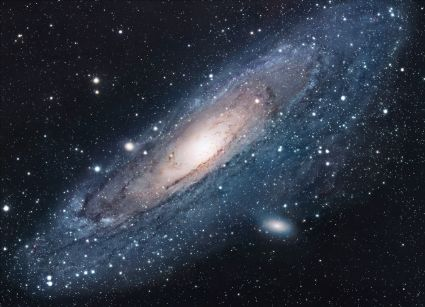
\includegraphics{universe.jpg} % its best practice to not inlcude file extension
% but I will here for VS Code

Theres a picture of the galaxy above.

\newpage
% Start of page 2

% Demo about how to add comments to images
\begin{figure}
    \centering
    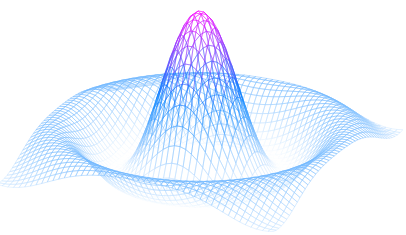
\includegraphics[width=0.75\textwidth]{mesh.png}
    % This form of \includegraphics instructs LaTeX to set the figure’s width to
    % 75% of the text width—whose value is stored in the \textwidth command.

    \caption{A nice plot.}
    % As its name suggests, this command sets the figure caption which can be
    % placed above or below the figure. If you create a list of figures this
    % caption will be used in that list.

    \label{fig:mesh1}
    % To reference this image within your document you give it a label using the
    % \label command. The label is used to generate a number for the image and,
    % combined with the next command, will allow you to reference it.
\end{figure}


As you can see in figure \ref{fig:mesh1}, the function grows near the origin.
% \ref{fig:mesh1}: This code will be substituted by the number corresponding to
% the referenced figure.
This example on the page \pageref{fig:mesh1}.

\newpage
% Start of page 3

% Demo of lists in LaTex %
Unordered lists
\begin{itemize}
    \item The individual entries are indicated with a black dot, a so-called
          bullet.

    \item The text in the entries may be of any length.
\end{itemize}

Ordered Lists
\begin{enumerate}
    \item This is the first entry in our list.
    \item The list increase with each entry we add.
\end{enumerate}


\newpage
% Start of page 4

% Will start doing a demo about how math works in LaTex
% There is inline math, where math is shown within text
% And there is display math, where it isn't part of the text or pargraph
In physics, the mass-energy equivalence is stated by the equation $E=mc^2$,
discovered in 1905 by Albert Einstein.
% This is an example of inline math. You have to use one of the delimiters like
% \( ... \), $ ... $ or \begin{math} ... \end{math}

% Here is some more examples of its usage
\begin{math}
E = mc^2
\end{math} is typeset in a pargraph using inline math mode---as is $E=mc^2$ and
so too is \(E=mc^2\).

% Here is for display math, where is can be enumerated or not
The mass-energy equivalence is described by the famous equation \[E=mc^2\]
discovered in 1905 by Albert Einstein.

In natural units ($ c=1 $), the formula expresses the identity
\begin{equation}
    E=m
\end{equation}



\end{document}
%               %
%  End Document %
%               %